\documentclass[11pt,a4paper]{article}
\usepackage{hyperref}
\usepackage{graphicx}
\begin{document}
\begin{titlepage}
\title{\textbf{Software Requirements Specification}\\Computer Science Marks System\\ \small Version: 0.3\\ \url{https://github.com/erosslee/COS301_MiniProject}}

\author{\textit{By group 10:} \\Estian Rosslee 12223426\\Moeletji Semenya 12349136\\Thulasizwe Mavuso 29236259\\Uteshlen Nadesan 28163304\\Zenadia Groenewald 12265676\\Z\"uhnja Riekert 12040593\\ \\
\textit{For:} \\Mr. Jan Kroeze (University of Pretoria)}



\maketitle
\end{titlepage}
\pagebreak
\tableofcontents
\pagebreak
\section{Introduction}
\textbf{(NOT DONE Zenadia said she'll do this part)}\\ \\


\section{Vision}
\textbf{(DONE by Z\"uhnja - needs to be checked)}\\ \\
The main purpose of this project is that marks can easily be added directly to the university\textquoteright
s database through a user-friendly interface. No in between procedures.   Evaluators will be able to access the system with a mobile approach or via computer while they are assessing.  Students will be able to log into the system and view all of their marks. \\ \\
The client\textquoteright
s main aim with this project is to simplify and increase the efficiency of the marking system.

\section{Background}
\textbf{(DONE by Z\"uhnja - needs to be checked)}\\ \\
Currently students view their marks for COS modules once it is posted on the CS-site.  It is usually listed according to their student numbers.  Thus students are able to view each other\textquoteright s marks.  \\ \\
During COS practical evaluations, markers evaluate each student\textquoteright s work and write their marks down on paper.  That then has to be passed to someone who has the time to enter the marks into the University\textquoteright s system.  In the process of this marking system the marks can easily get lost. \\ \\
This project eliminates these threats.  Marks won\textquoteright t have the opportunity to get lost, since it will be added to the system immediately. Students will be able to immediately access their marks once it is added to the system and they won\textquoteright t be able to view any marks that are not their own. 

\section{Stakeholders}
The stakeholders invloved in this project are: 
\begin{itemize}
\item Mr. Jan Kroeze and the Department of Computer Science(client). 
\item Students and lecturers at the Department(end-users).
\item COS 301 students of 2014(developers).
\item University of Pretoria(organization). 
\end{itemize}

\section{Architectural requirements}
\textbf{(DONE by Thulasiswe - needs to be checked)}\\ \\
\subsection{Access channel requirements}
The system's services are to be accessed by Android application clients and Browser clients through its web interface. These are the only two platforms that are to be supported by the system.
\subsection{Quality requirements}
\subsubsection{Performance}
	\begin{itemize}
	\item System must not take more than 1.5 seconds to return a searched for student.
	\item A request to view marks must be granted within 1.2 seconds.
	\item System must have auto complete mechanism for search services.
	\end{itemize}

	\subsubsection{Audit-ability}
	\begin{itemize}
	\item Every action on the system must be recorded on a log that can later be viewed and queried.
	\item Actions that are to be recorded
	\begin{itemize}
	\item The current user performing the action.
	\item New mark capturing.
	\item Deletion of marks.
	\item Edition of marks.
	\item Reason for editing the marks.
	\item The date/time on which an action was performed.
	\end{itemize}
	\end{itemize}

\subsubsection{Scalabity}
	\begin{itemize}
	\item The system must be able to be accessed by up to the current number of students registered for the course at any point.
	\item Additions and updates must be available to all the TA's when a mark sheet is unlocked.
	\end{itemize}	

	\subsubsection{Authorization}
	\begin{itemize}
	\item All actions are granted to a user based on the privileges they have.
	\end{itemize}

	\subsubsection{Authentication}
	\begin{itemize}
	\item The system must have an access control mechanism.
	\item Access control must be handled at log in/out points.
	\end{itemize}


\subsection{Integration requirements}
\textbf{(NOT DONE - Who will do this?)}\\ \\
\subsection{Architectural constraints}
\textbf{(DONE by Thulasiswe - needs to be checked)}\\ \\
\subsubsection{Technologies to be used}
	\begin{itemize}
	\item For the application platform
	\begin{itemize}
	\item Android SDK
	\item Java
	\end{itemize}
	\item For the web interface
	\begin{itemize}
	\item JavaScript
	\item HTML 4.0/HTML 5
	\end{itemize}
	\item Must be secure therefore must run over HTTPS
	\item Server-side
	\begin{itemize}
	\item Django framework
	\item Python
	\end{itemize}
	\item Web service
	\begin{itemize}
	\item SOAP
	\end{itemize}
	\item MySQL for database
	\item LDAP for distributed directory information service
	\end{itemize}

\section{Functional requirements}
\subsection{Introduction}
The function of this project is to design an application interface that would enable a marker to upload the mark of a student, in a practical session, with his/her phone.
\subsection{Scope and Limitations/Exclusions}
\textbf {Use a high-level use case diagram with}\\
\subsubsection{Scope}
\textbf {Phone interface for the marker}

\begin{itemize}
\item Markers should only be able to view students who have registered for the specific practical period the marker is assigned to.
\item On specific markers with specific credentials should be able to log on to the application.
\item Markers can only log onto the application for their’ specified time slot and the application should run a check to provide this.
\item The marker should be able to look up the student being marked on his/her phone with either a student number or a first, last or both the first and last names of the student.
\item The interface should be simplistic and show the rubric and mark layout and have input boxes for the different mark fields.
\item For a change of a mark, the marker must provide a reason in the textbox that is saved for future reference.
\end{itemize}
\textbf{A web interface is also needed for lecturers and students}\\\\
\textbf{Lecturers:}

\begin{itemize}
\item Can only view records for courses they are in charge of.
\item Need to be able to view records of marks as well as specific marks.
\item PDF documents for Lecturers should be generated detailing marks and 
descriptions.
\item Graphs of students’ marks should also be generated in the form of normal 
distributions, bar graphs and pie charts.
\item Counts of students should be available, as well as students registered standard 
deviations, averages and medians.
\end{itemize}
\textbf{Students:}
\begin{itemize}
\item Students should only be allowed to view their’ own marks and check their progress in the course thus far as well as overall progress with the course.
\item The student should not be able to edit marks.
\end{itemize}




\subsubsection{Limitations/Exclusions}


List the exclusions/limitations, discussing any functionality which could erroneously be assumed within scope but which has been explicitly excluded from the scope of the system.
\subsection{Required functionality}
\textbf{This application should be:}

\begin{itemize}
\item Accessible on android phones.
\item Scalable and viewable on devices.
\item Secure and information sent and received should be encrypted.
\item Auto log out after a specified time.
\end{itemize}

\textbf{The application:}
\begin{itemize}
\item Should have a database containing all students, lecturers and administrators as well as markers and a root user.
\item The root user should have access to all fields of the database. 
\item Should integrate with the automatic marker Fitchfork to receive specific student marks and be able to add these marks to a students’ mark database.
\item Should auto-complete names and student numbers being entered by markers. 
\item Generate CSV files for viewing and also be able to accept CSV files of marks for input into the database of students marks.

\end{itemize}

\subsection{Use case prioritization}

\subsubsection{Critical: }
\begin{itemize}
\item The application needs to be functioning on the android platform and should be available on all android phones for android version 2.0 upwards.
\item Marks must be able to be entered and uploaded to the server.
\item Have a web interface for viewing marks for students.
\item have a web interface specific for lecturers.
\item Fitchfork integration.
\end{itemize}

\subsubsection{Important: } 
\begin{itemize}
\item Good to exceptional performance speeds.
\item Encryption of communications.
\item Have a root user with unlimited access to the database and application. (The root user cannot edit audit-able documents)
\item Generated PDF documents with detailed reports.
\end{itemize}
\subsubsection{Nice-To-Have} 
\begin{itemize}
\item Auto-Complete.
\item Auto log off.
\item Student search via first name and/or surname.
\end{itemize}

\subsection{Use case/Services contracts}
For each use case/service specify
\\\\
\textbf{Pre-Conditions: }the conditions under which the service may be refused (usually there is an exception associated with each pre-condition).
\\\\
\textbf{Post-Conditions: }the conditions which must hold true after the service has been provided.
\\\\
\textbf{Request and Results Data Structures: }Use class diagrams to specify the data structure requirements for the request and result objects (i.e. the inputs and outputs).
\subsection{Process specifications}
For some of the use cases there may be requirements around the process which needs to be followed. If so, these requirements are typically specified via activity and/or sequence diagrams or
alternatively via state charts.
\subsection{Domain Objects}
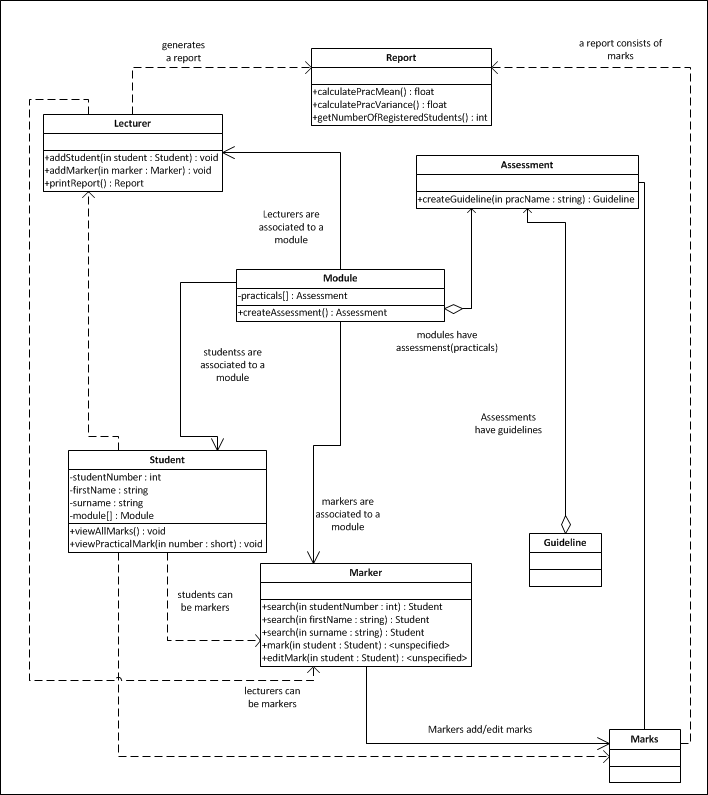
\includegraphics[width=1.0\linewidth]{Class_Diagram}
\\\\
Above is a class digram of the system with classes that contain attributes and methods in order to make the relatioships clearer to understand. 
\section{Open Issues}
Discuss in this section
\begin{itemize}
\item any aspects of the requirements which still need to be specified,
\item around which clarification is still required, as well as
\item any discovered inconsistencies in the requirements.
\end{itemize}
\section{Glossary}
The requirements is to be read, understood and validated by a range of people from very different backgrounds (the client, domain experts/business analysts, the developers, software architects, users, ... ). Use a glossary to explain any terms which some parties may not be familiar with.
\end{document}
